\newpage
\setcounter{section}1
\section{Overall description}
\subsection{Product Perspective}
\quad Our product is a web application that mainly focuses on events and their weather forecast information. It is a stand-alone product that is not depend on a larger system or included in one. It mainly consists of two parts: front-end and back-end. While front-end is responsible for providing all product functionalities to the user with useful, smooth and easy interfaces, back-end is responsible for managing all functionalities and communicating with the front-end in order to provide the best experience to the users.

\subsubsection{System Interfaces}
\quad There are no system interfaces provided by our product.

\subsubsection{User Interfaces}
\quad There are mainly five different user interfaces, these are register, login, edit event, edit profile, create event, and last but not least view calendar page. These pages will be explained in detail in later sections.
\begin{figure}[tbh]
  \begin{center}
  % Requires \usepackage{graphicx}
  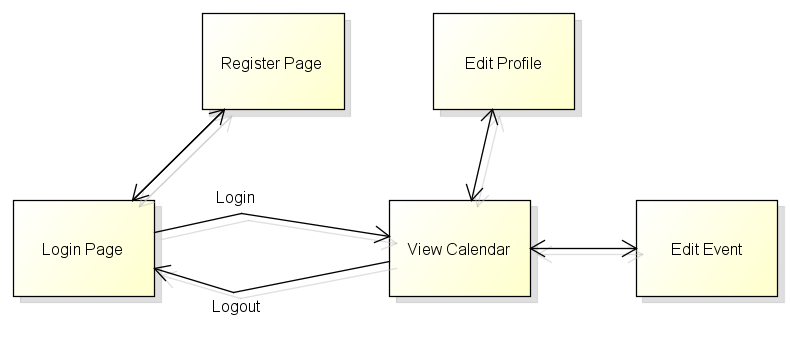
\includegraphics[width=150mm]{Flowchart0}
    \label{Fig 1:}
  \end{center}
\end{figure}
\newpage
\subsubsection{Hardware Interfaces}
\quad There are no hardware interfaces provided by our product.

\subsubsection{Software Interfaces}
\quad Our application will be written with EJB (Enterprise Java Beans) framework, that means it will work with the JVM (Java Virtual Machine). Therefore, there are no specific operating system requirement. The application will work on the Glassfish Server v4.1. The required database system is MySQL with the version number 5.6.17.

\subsubsection{Communication Interfaces}
\quad The MySQL server and our back-end communicates on the port 3306. Glassfish server uses the 8080 port for HTTP requests. The database and the server locate always at the same physical address.

\subsubsection{Memory}
\quad The system should have at least 1 GB of primary memory and have at least 10 GB of free secondary memory space.

\subsection{Product Functions}
\quad Our project provides users an opportunity to schedule their events by means of weather forecast information. By using the WeCalEvent system, users can edit and postpone their events if there exist a weather condition with which they are not willing to host their events. In addition to that, users are able to invite other users of the system to their events. System will notify the every participant user of the event in case of weather forecast change and suggest a better day to the event owner.
\par The first actor of the project is the user. However, the users may have different roles on the system depending on their relation with the event. There are basically three different roles:
\begin{itemize}
  \item Event owner: This user can edit the event and can invite other users.
  \item Invited user: This user can accept or reject the invitation.
  \item Participant user: This user is able to see the event details even if it is private and receives notifications about the event.
\end{itemize}
\par The second actor is the system. System checks periodically whether the forecast is changed or not. It has the responsibility of notifying the users via application and e-mail.
\newpage
\begin{figure}[tbh]
  \begin{center}
  % Requires \usepackage{graphicx}
  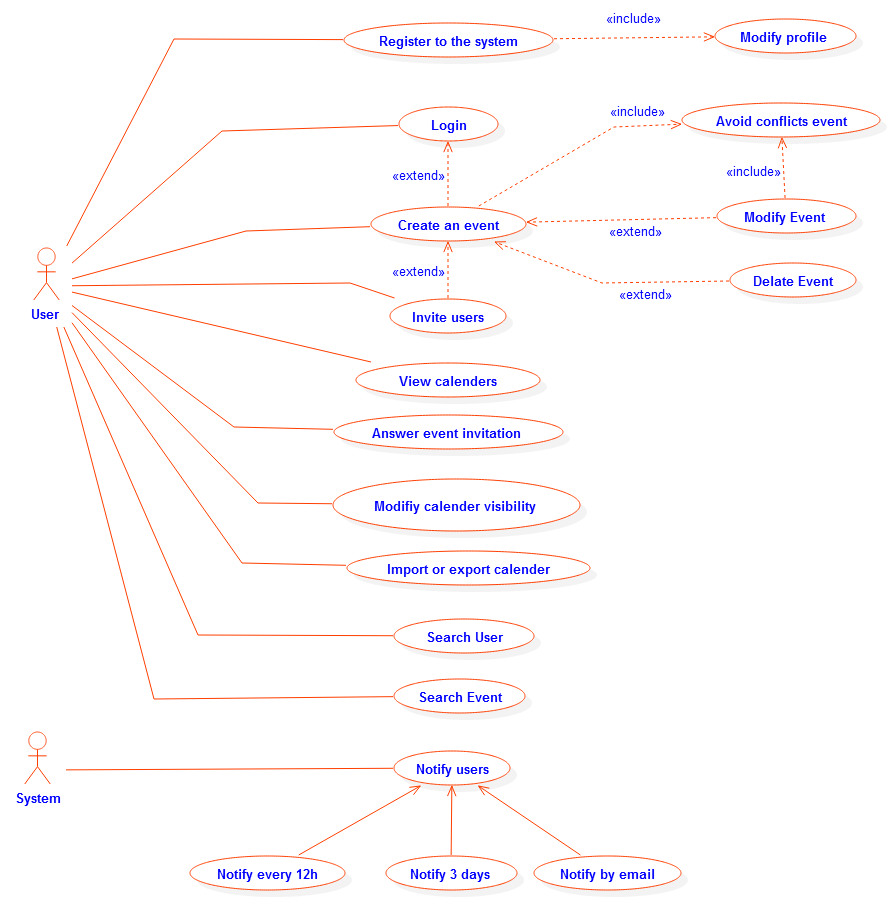
\includegraphics[width=160mm]{UseCases}
  \caption{Use Cases}\label{Fig 2:}
  \end{center}
\end{figure}

%\subsection{User Characteristics}
\subsection{Constraints}
\quad The system is constrained by the server machine on which our application works. The forecast information is constrained by the external system used for weather forecast. Furthermore, the internet constraints the application because the weather data is derived from the internet as the web interface is requested via HTTP Request through Internet.
\subsection{Assumptions}
\quad The weather forecast is provided for the next 16 days. If a user is creating an event within this period of time and the weather is not good for the event on the chosen date the user will still be able to create an event on this date. In this case he will be notified that the weather conditions do not match the needed ones.
\par The event organiser will be notified if the weather is "bad" 3 days before the event. If there is no "good" weather within next 13 days we notify user but we cannot suggest any other day .
\par The event creator can choose which weather conditions to be warned about. The weather conditions list is: cloudy, rainy, snowy, sunny, unknown.
\par The event organiser will be able to invite users after the event creation.